\documentclass[9pt,twocolumn,twoside,lineno]{pnas-new}
% Use the lineno option to display guide line numbers if required.
% Note that the use of elements such as single-column equations
% may affect the guide line number alignment. 

%%Nadir's Shortcuts
\newcommand{\beqn}{\begin{equation}}
\newcommand{\eeqn}{\end{equation}}
\newcommand{\beqa}{\begin{eqnarray}}
\newcommand{\eeqa}{\end{eqnarray}}
\newcommand{\beqanonum}{\begin{eqnarray*}}
\newcommand{\eeqanonum}{\end{eqnarray*}}
\newcommand{\beqnonum}{\begin{equation*}}
\newcommand{\eeqnonum}{\end{equation*}}
\newcommand{\jump}{\vspace{0.5cm}}
\newcommand{\bbf}{\begin{bf}}
\newcommand{\ebf}{\end{bf}}
\newcommand{\eqnref}[1]{(\ref{#1})}
\newcommand{\defn}[1]{\begin{bf}\emph{#1}\end{bf}}
\newcommand{\reals}{\ensuremath{\mathbb{R}}}
\newcommand{\complex}{\ensuremath{\mathbb{C}}}
\newcommand{\integers}{\ensuremath{\mathbb{Z}}}
\newcommand{\half}{\ensuremath{\frac{1}{2}}}
\newcommand{\n}{\nonumber}
\newcommand{\inverse}{^{-1}}

%calculus shorthand
\newcommand{\timeder}{\frac{d}{dt}}
\newcommand{\partialder}[1]{\frac{\partial}{\partial #1}}
\newcommand{\partialderf}[2]{\ensuremath{\frac{\partial #1}{\partial #2}}}
\newcommand{\der}[2]{\ensuremath{\frac{d #1}{d #2}}}
\newcommand{\dx}{\ensuremath{\frac{d}{dx}}}
\newcommand{\ddx}{\ensuremath{\frac{d}{dx}}}
\newcommand{\kvec}{\ensuremath{\vec{k}}}
\newcommand{\uvec}{\ensuremath{\mathbf{u}}}
\newcommand{\zhat}{\ensuremath{\mathbf{\hat{z}}}}
\newcommand{\khat}{\ensuremath{\mathbf{\hat{k}}}}
\newcommand{\unitvect}[1]{\ensuremath{\mathbf{\hat{#1}}}}
\newcommand{\ppx}{\ensuremath{\partial_x}}
\newcommand{\ppy}{\ensuremath{\partial_y}}
\newcommand{\ppz}{\ensuremath{\partial_z}}
\newcommand{\ppt}{\ensuremath{\partial_T}}
\newcommand{\ppp}{\ensuremath{\partial_p}}


% radiation shorthand
\newcommand{\cotwo}{\ensuremath{\mathrm{CO_2}}}
\newcommand{\othree}{\ensuremath{\mathrm{O_3}}}
\newcommand{\htwo}{\ensuremath{\mathrm{H_2O}}}
\newcommand{\QLW}{\ensuremath{Q_\mathrm{LW}}}
\newcommand{\QSW}{\ensuremath{Q_\mathrm{SW}}}
\newcommand{\Qnet}{\ensuremath{Q_\mathrm{net}}}
\newcommand{\FLW}{\ensuremath{F^\mathrm{LW}}}
\newcommand{\FSW}{\ensuremath{F^\mathrm{SW}}}
\newcommand{\FLWgl}{\ensuremath{F^\mathrm{LW}_{\mathrm{gl}}}}
\newcommand{\FSWgl}{\ensuremath{F^\mathrm{SW}_{\mathrm{gl}}}}
\newcommand{\USW}{\ensuremath{U^\mathrm{SW}}}
\newcommand{\DSW}{\ensuremath{D^\mathrm{SW}}}
\newcommand{\Fnet}{\ensuremath{F^\mathrm{net}}}
\newcommand{\Fnetgl}{\ensuremath{F^\mathrm{net}_{\mathrm{gl}}}}
\newcommand{\Fgl}{\ensuremath{F_{\mathrm{gl}}}}
\newcommand{\olr}{\ensuremath{\mathrm{OLR}}}
\newcommand{\OLR}{\ensuremath{\mathrm{OLR}}}
\newcommand{\trans}{\ensuremath{\mathcal{T}}}
\newcommand{\solar}{\ensuremath{I_0}}
\newcommand{\cool}{\ensuremath{\mathcal{C}}}
\newcommand{\cminverse}{\ensuremath{\mathrm{cm^{-1}}}}
\newcommand{\pierre}{P10}
\newcommand{\tauk}{\ensuremath{\tau_\lambda}}

% Units
\newcommand{\Wmsq}{\ensuremath{\mathrm{W/m^2}}}
\newcommand{\meter}{\ensuremath{\mathrm{m}}}
\newcommand{\kg}{\ensuremath{\mathrm{kg}}}
\newcommand{\Kinverse}{\ensuremath{\mathrm{K^{-1}}}}
\newcommand{\Kelvin}{\ensuremath{\mathrm{K}}}

% meteorology shorthand
\newcommand{\qv}{\ensuremath{q}}
\newcommand{\rhov}{\ensuremath{\rho_\mathrm{v}}}
\newcommand{\Hv}{\ensuremath{H_\mathrm{v}}}
\newcommand{\Rv}{\ensuremath{R_\mathrm{v}}}
\newcommand{\qa}{\ensuremath{q_a}}
\newcommand{\qvstar}{\ensuremath{q^*}}
\newcommand{\pvstar}{\ensuremath{p^*_{\mathrm{v}}}}
\newcommand{\Ta}{\ensuremath{T_a}}
\newcommand{\Tav}{\ensuremath{T_\mathrm{av}}}
\newcommand{\Ts}{\ensuremath{T_\mathrm{s}}}
\newcommand{\Tsgl}{\ensuremath{T_\mathrm{s,gl}}}
\newcommand{\ps}{\ensuremath{p_s}}
\newcommand{\RH}{\ensuremath{\mathrm{RH}}}
\newcommand{\cld}{\ensuremath{\mathrm{Cld}}}
\newcommand{\WVP}{\ensuremath{\mathrm{WVP}}}
\newcommand{\ztop}{\ensuremath{z_\mathrm{top}}}
\newcommand{\ztp}{\ensuremath{z_\mathrm{tp}}}
\newcommand{\zlcl}{\ensuremath{z_\mathrm{LCL}}}
\newcommand{\Tlcl}{\ensuremath{T_\mathrm{LCL}}}
\newcommand{\Ttp}{\ensuremath{T_\mathrm{tp}}}
\newcommand{\ptp}{\ensuremath{p_\mathrm{tp}}}
\newcommand{\lapseav}{\ensuremath{\Gamma_\mathrm{av}}}
\newcommand{\gammaav}{\ensuremath{\Gamma_\mathrm{av}}}
\newcommand{\Htauk}{\ensuremath{H_{\tau_k}}}
\newcommand{\east}{\ensuremath{\mathrm{E}}}
\newcommand{\north}{\ensuremath{\mathrm{N}}}
\newcommand{\south}{\ensuremath{\mathrm{S}}}
\newcommand{\tav}{\ensuremath{t_\mathrm{av}}}
\newcommand{\kmax}{\ensuremath{k_\mathrm{max}}}
\newcommand{\kmin}{\ensuremath{k_\mathrm{min}}}

%Variables
\newcommand{\figurepath}{../../figures/}



\templatetype{pnasresearcharticle} % Choose template 
% {pnasresearcharticle} = Template for a two-column research article
% {pnasmathematics} = Template for a one-column mathematics article
% {pnasinvited} = Template for a PNAS invited submission

\title{Mean Precipitation Change from a Deepening Troposphere}

% Use letters for affiliations, numbers to show equal authorship (if applicable) and to indicate the corresponding author
\author[a,b,c]{Nadir Jeevanjee}
\author[d,e]{David M. Romps} 


\affil[a]{Department of Geosciences, Princeton University, Princeton NJ 08544 USA}
\affil[b]{Princeton Program in Atmosphere and Ocean Sciences, Princeton University, Princeton NJ 08540 USA}
\affil[c]{Geophysical Fluid Dynamics Laboratory,  Princeton NJ  08540 USA}
\affil[d]{Department of Earth and Planetary Sciences, University of California at Berkeley, Berkeley, CA 94702  USA}
\affil[e]{Climate and Ecosystems Science Division, Lawrence Berkeley National Laboratory, Berkeley, CA USA}

% Please give the surname of the lead author for the running footer
\leadauthor{Jeevanjee} 

% Please add here a significance statement to explain the relevance of your work
\significancestatement{Global climate models robustly predict that global mean precipitation should increase at roughly 2-3 \% \Kinverse, but the origin of these values is not well understood. Here we develop a simple theory to help explain these values. This theory suggests that global mean precipitation is closely tied to the depth of the troposphere, when measured in temperature coordinates. When surface temperatures increase, this `temperature depth' of the troposphere also increases, causing an increase in global mean precipitation.}

% Please include corresponding author, author contribution and author declaration information
\authorcontributions{N.J. and D.M.R. designed research and analyzed data. N.J. wrote the paper.}
\authordeclaration{The authors declare no conflict of interest.}
%\equalauthors{\textsuperscript{1}}
\correspondingauthor{\textsuperscript{2}To whom correspondence should be addressed. E-mail: nadirj\@princeton.edu}

% Keywords are not mandatory, but authors are strongly encouraged to provide them. If provided, please include two to five keywords, separated by the pipe symbol, e.g:
\keywords{Climate Change $|$ Atmospheric Science $|$ Hydrological Cycle $|$} 

\begin{abstract}
Global climate models robustly predict that global mean precipitation should increase at roughly 2-3 \% \Kinverse, but the origin of these values is not well understood. Here we develop a simple theory to help explain these values, in the simplified context of cloud-resolving simulations of the tropical atmosphere. Our theory combines the well-known radiative constraint on precipitation, which says that condensation heating from precipitation is balanced by the net radiative cooling of the atmosphere, with a  universality of radiative cooling profiles when expressed in temperature coordinates. These two constraints yield a picture in which mean precipitation is controlled primarily by the depth of the troposphere, when measured in temperature coordinates. This yields quantitative insight into the 2-3 \% \Kinverse\ increase in mean precipitation exhibited by our simulations.  The relevance of our results to global climate simulations is also assessed. \end{abstract}

\dates{This manuscript was compiled on \today}
\doi{\url{www.pnas.org/cgi/doi/10.1073/pnas.XXXXXXXXXX}}

\begin{document}

% Optional adjustment to line up main text (after abstract) of first page with line numbers, when using both lineno and twocolumn options.
% You should only change this length when you've finalised the article contents.
\verticaladjustment{-2pt}

\maketitle
\thispagestyle{firststyle}
\ifthenelse{\boolean{shortarticle}}{\ifthenelse{\boolean{singlecolumn}}{\abscontentformatted}{\abscontent}}{}
% If your first paragraph (i.e. with the \dropcap) contains a list environment (quote, quotation, theorem, definition, enumerate, itemize...), the line after the list may have some extra indentation. If this is the case, add \parshape=0 to the end of the list environment.
%\dropcap{T}his PNAS journal template is provided to help you write your work in the correct journal format.  Instructions for use are provided below.
%
%Note: please start your introduction without including the word ``Introduction'' as a section heading (except for math articles in the Physical Sciences section); this heading is implied in the first paragraphs. 
Despite its fundamental role in driving atmospheric motions, atmospheric radiative cooling remains somewhat enigmatic. Though the fundamentals of radiative transfer are quite well-understood and have been for some time, translating these fundamentals into realistic cooling rates requires a symphony of complicated spectroscopic and radiative transfer calculations which render the final result somewhat inscrutable. As a result, we lack simple descriptions of the radiative cooling profiles produced by our numerical models.

One implication of this is that quantities that are closely tied to radiative cooling, such as global mean precipitation, also remain somewhat enigmatic. We do know that the atmospheric (rather than planetary) energy budget, in which condensation heating from precipitation balances atmospheric radiative cooling, constrains global mean precipitation $P$ to be roughly equal to column-integrated net radiative cooling $\Qnet$ \cite{ogorman2012,allen2002}:
\beqn
	LP \approx \Qnet \quad \mbox{(\Wmsq)} \label{rad_precip_constraint}
\eeqn
(here $L$ is the latent heat of vaporization and we neglect surface sensible heat fluxes, a point we return to below). We also know that  global climate models robustly exhibit  mean precipitation increases with warming of $2 -3\%\ \Kinverse$  \cite{stephens2008a, lambert2008, held2006}. Furthermore, recent work \cite{stephens2010, pendergrass2014, takahashi2009}  has explained this increase in global mean precipitation in terms of an increase in downward radiative emission from the atmosphere at the surface. Despite this progress, however, a basic question remains unanswered: why does this increase take on the value that it does? Why $2 -3\%\ \Kinverse$ and not many times  larger or smaller?

This paper aims to reveal some simple behavior in radiative cooling profiles, and to use it to  answer this question about precipitation change. We will  focus on how vertically-resolved radiative cooling profiles change with warming, rather than focusing on radiative fluxes at the surface or top-of-atmosphere. In particular, we will argue, following \cite{simpson1928} and \cite{ingram2010}, that water vapor density and optical depth profiles should behave very simply when considered as functions of temperature as a vertical coordinate. This then implies  that LW and SW radiative flux divergences should also behave simply in temperature coordinates. This simple behavior leads to a predictive expression for $d\Qnet/d\Ts$ and hence $dP/d\Ts$ (\Ts\ is surface temperature), which we validate with limited-area cloud-resolving model (CRM) simulations which emulate  the tropical atmosphere. We then seek insight from our results, and also ask to what extent they generalize to global climate models (GCMs). 


This approach leverages the insights of \cite{simpson1928, ingram2010}, but also builds upon their work in various ways. First, we verify some of their ideas using comprehensive radiative transfer calculations, which to our knowledge has not yet been done. We also shift the focus from outgoing longwave radiation (i.e., thermal emission to space) to atmospheric radiative cooling, and also extend their  arguments to include both the longwave (LW, thermal emission) and shortwave (SW, solar radiation) bands. Our work also has precedent in \cite{takahashi2009}, which also takes an idealized approach in analyzing the radiative constraint on hydrological sensitivity. That study, however,  used a gray radiation model wherein the concentration of the longwave absorber is not directly tied to temperature, a  link which will prove crucial here (see Eqns. \ref{rhov}-\ref{tauT} below).

\section{CRM Simulations of RCE}
We will study precipitation change in one of the simplest systems in which the radiative constraint on precipitation \eqnref{rad_precip_constraint} operates, namely cloud-resolving radiative-convective equilibrium (RCE) with fixed sea-surface temperature. This system approximates the real tropics, where the majority of Earth's precipitation occurs \cite{simpson1988}, and exhibits precipitation increases of roughly $3 -4\%\ \Kinverse$, similar to the GCM range \cite{romps2011, muller2011b}.  

We simulate RCE using Das Atmosph\"arische Modell \cite[DAM,][]{romps2008}, a fully-compressible, non-hydrostatic cloud-resolving model, coupled to radiation via the comprehensive Rapid Radiative Transfer Model 
\cite[RRTM,][]{mlawer1997}. DAM employs the six-class Lin-Lord-Krueger  microphysics scheme \cite{lin1983, lord1984, krueger1995}, and in contrast to the original formulation in \cite{romps2008} employs no explicit sub-grid scale turbulence scheme, relying instead on `implicit LES'  \citep[][essentially just the existing numerical diffusion]{margolin2006}  for sub-grid scale transport.

%Figure rhov_fig
\begin{figure}[t]
	\begin{center}
			\includegraphics[scale=0.4]{\figurepath rhov.pdf}
		\caption{Profiles of $\rhov(T)$ from our RCE simulations at various \Ts, with both linear and log scales. These profiles are `\Ts-invariant' in the sense that $\rhov(T)$ does not depend on \Ts, i.e. that the \rhov\ profiles at different \Ts\ collapse onto a single curve.
		\label{rhov_fig}
		}
	\end{center}
\end{figure}

	
	Our RCE simulations ran on a square doubly-periodic domain of horizontal dimension $L=72$ km, with  a horizontal resolution of $dx=1$ km. The vertical grid stretched smoothly from 50 m resolution below 1000 m to 250 m resolution between 1000 m and 5000 m, and then to 500 m up to the model top at  30 km. We calculated surface heat and moisture fluxes using simple bulk aerodynamic formulae, and used a pre-industrial \cotwo\  concentration of 280 ppm with no ozone. To explore precipitation changes  with warming we ran five experiments at surface temperatures of $\Ts=(280,290,300,310,320)$ K, though many of our figures omit the 320 K run for clarity. Our runs branched off the equilibrated runs described in \cite{romps2014}, and were run for 60 days  to iron out any artifacts from changing the domain and resolution. All vertical profiles are time-mean and domain-mean, averaged over the last 20 days of each run. 
	
Since we run with prescribed \Ts\ and fixed \cotwo, we are isolating the hydrological sensitivity to \Ts\ and neglecting the rapid adjustment from \cotwo.  Recent work has shown that the former is relatively robust across models and is also robust to forcing type, whereas rapid adjustments depend on the forcing type \cite{flaschner2016,samset2017}. The rapid adjustment to \cotwo\ contributes roughly -1 \Wmsq/K \cite{pendergrass2014}, a non-negligible but still sub-dominant effect. 

%=================================%
% Temperature invariance of flux divergence %
%=================================%
\section{\Ts-invariance of Flux Divergences}
\label{Ts_invariance}
The simple behavior of radiative cooling alluded to above begins with the key fact that  the water vapor density 
	\beqn
		\rhov =  \RH\frac{\pvstar(T)}{\Rv T} \; 
	\label{rhov}
	\eeqn
	 is (up to variations in relative humidity \RH) a function of temperature only. [Note that it has been shown recently that RH is itself a function of $T$ in RCE \cite{romps2014}. Also note that here $p_v^*$  is the saturation vapor pressure of water, and all other symbols have their usual meaning.] If we use $T$ as a vertical coordinate,  Eqn. \eqnref{rhov} then tells us that the function $\rhov(T)$ does not depend on \Ts. This is what we mean by `\Ts-invariance'. We verify \Ts-invariance of $\rhov(T)$  in Fig. \ref{rhov_fig}, where indeed  the \rhov\ profiles at different \Ts\ collapse onto a single curve when plotted in temperature coordinates.


	%Figure pptflw_tinv_dam
\begin{figure}[t]
	\begin{center}
			\includegraphics[scale=0.3]{\figurepath pptflw_tinv_dam.pdf}
		\caption{LW flux divergence  $-\ppt \FLW$, as diagnosed from RRTM coupled to our CRM RCE simulations at \Ts=(280,\ 290,\ 300,\ 310) K. Fluxes are plotted from the lifting condensation level of each simulation to 22.5 km for clarity, and  in height, pressure, and temperature coordinates to emphasize the \Ts-invariance of  $(-\ppt \FLW)(T)$. The gray dotted line in the right panel plots $-\ppt \FLW = 0$, and shows the \Ts-invariance of $\Ttp \approx 185$ K.
		\label{pptflw_tinv_dam}
		}
	\end{center}
\end{figure}

	 
	For wavelengths  $\lambda$ where water vapor dominates, the optical depth $\tauk$ is just
	\beqn
		\tauk(z) = \kappa(\lambda) \int_z^\infty   \rhov(z') \, dz'  \; 
		\label{tauz}
	\eeqn
		where $\kappa(\lambda)$ is a  mass absorption coefficient  (units $\mathrm{m^2/kg}$) whose pressure-broadening we neglect \citep[as in][see  also section \ref{sec_summary}]{ingram2010}. Note that optical depth itself is dimensionless, and can be interpreted as the ratio of the total effective area of absorbers in a column (above a given height) to the actual area of the column. Changing the integration variable in Eqn. \eqnref{tauz} to temperature $T'$  yields
		\beqn
		\tauk(T) \approx  \kappa(\lambda) \int_{\Ttp}^T   \rhov(T') \, \frac{dT'}{\Gamma}  \; ,
		\label{tauT}
	\eeqn
	where we neglect stratospheric water vapor and take the lower limit of the integral to be the tropopause temperature $\Ttp \approx 185$ K, where radiative cooling goes to 0 (see Figs. \ref{pptflw_tinv_dam} and  \ref{pptfsw_tinv_dam}, which also show that \Ttp\ is \Ts-invariant). The only quantity in Eqn. \eqnref{tauT} that might still exhibit some \Ts-dependence is the  moist lapse rate $\Gamma\equiv -\frac{dT}{dz}$, but Figure 2 of \cite{ingram2010} shows that when $\Gamma$ is considered a function of temperature, it too is fairly  \Ts-invariant. Equation \eqnref{tauT} then implies that \tauk\ profiles at any $\lambda$ exhibit the same \Ts-invariance as \rhov. This argument was also made by \cite{ingram2010}, and its essence goes back to  \cite{simpson1928}.
	
	To build on this and connect it with radiative cooling, we invoke the cooling-to-space  approximation \cite[][]{thomas2002, rodgers1966}, which says that the spectrally resolved LW flux divergence in temperature coordinates $-\ppt \FLW_\lambda$ (units $\Wmsq/\mathrm{K}/\meter$, fluxes positive upward, minus sign introduced to maintain a consistent sign with  $\ppz \FLW_\lambda$) is approximately
	\beqn
		-\ppt \FLW_\lambda \approx - \pi B_\lambda(T) \frac{d (e^{-\tauk(T)})}{dT} \ ,
	\label{cts_spectral}
	\eeqn
where  the transmission function $e^{-\tauk}$ gives the fraction of radiation emitted at a given height that travels unabsorbed out to space. (Note that RRTM does not employ \eqnref{cts_spectral}; we simply use it here as a heuristic.) Since the Planck function $B_\lambda(T)$ is \Ts-invariant, and the optical depth $\tauk(T)$ is as well, we also expect $-\ppt \FLW_\lambda$ to be \Ts-invariant. Since this holds for all wavelengths $\lambda$ where water vapor dominates, it should also hold approximately for the spectrally integrated LW flux divergence $-\ppt \FLW$ ($\Wmsq/\mathrm{K}$). This is confirmed in  Fig.  \ref{pptflw_tinv_dam}, which plots $(-\ppt \FLW)(T)$ as diagnosed from RRTM coupled to our  RCE simulations.  That figure also plots $-\ppt \FLW$ as functions of $z$ and $p$, to emphasize that this invariance only holds  when $T$ is used as the vertical coordinate.
	%Figure pptfsw_tinv_dam
\begin{figure}[t]
	\begin{center}
			\includegraphics[scale=0.3]{\figurepath pptfsw_tinv_dam.pdf}
		\caption{As in Fig. \ref{pptflw_tinv_dam}, but for SW instead of LW.
		\label{pptfsw_tinv_dam}
		}
	\end{center}
\end{figure}


	A similar argument holds for the SW flux divergence. If $I_\lambda$ is the incident solar flux at wavelength $\lambda$, and  neglecting reflection and scattering in the  near-infrared, 
%\cite[e.g.][]{frouin1990}, 
then  we have
	\beqn
		-\ppt \FSW_\lambda = - I_\lambda \der{(e^{-\tauk(T)})}{T}
		\
	\eeqn
\cite[][eqn. 9.26]{thomas2002}. This equation is similar to  \eqnref{cts_spectral} but with $B_\lambda(T) \rightarrow I_\lambda$, and since $I_\lambda$ is also \Ts-invariant, we can argue as above that $(-\ppt \FSW)(T)$ should be \Ts-invariant. This is confirmed in Fig. \ref{pptfsw_tinv_dam}, where again the simple behavior of $-\ppt \FSW$ in temperature coordinates is contrasted with that in height and pressure coordinates.



The fluxes used in Figs.  \ref{pptflw_tinv_dam} and \ref{pptfsw_tinv_dam} are all-sky fluxes (which include cloud radiative effects), but the foregoing argument was for clear-sky fluxes. This is permissible because cloud fractions in our RCE simulations are low (attaining a maximum of $\sim 10 \%$ at the anvil height in our simulations), so it is the clear-sky physics which dominates (Fig. S1). It is also possible that the \Ts-invariance demonstrated here benefits from the fixed temperature of anvil clouds \cite{hartmann2002,kuang2007,harrop2012}. We will touch upon cloud radiative effects further in section \ref{sec_GCMs}, when we assess how well these CRM results generalize to GCMs.
 
%=================%
% Simple picture for Q   %
%=================%
		
\section{A simple picture for column-integrated radiative cooling} \label{sec_simple_Q}

Now that we have established  the \Ts-invariance of radiative flux divergences, we can construct a simple, quantitative picture of how column-integrated radiative cooling, and hence precipitation,  changes with surface temperature. 
	
	Let $F$ denote radiative flux in a particular band -- LW, SW, or Net (LW+SW) -- and $Q$ the associated column-integrated free-tropospheric radiative cooling. We consider  the free troposphere (i.e. the troposphere above the planetary boundary layer), rather than the full troposphere, because the radiative constraint on precipitation 
		\beqn
			LP \approx \Qnet
		\label{p_constraint}
		\eeqn
		 holds best for the free troposphere  \cite{ogorman2012}. The underlying assumption is that surface sensible heat fluxes balance radiative cooling in the boundary layer, and so both can be eliminated from the atmospheric energy budget by considering the free troposphere. (This assumption was also made in \cite{takahashi2009}, and goes back to \cite{betts1989}.) We define the free troposphere here as being above the lifting condensation level \Tlcl\ where clouds begin to form and below the tropopause \Ttp.
	
	%Figure dqdts_cartoon
\begin{figure}[t]
	\begin{center}
			\includegraphics[scale=0.3,trim=0cm 0cm 0cm 5cm,clip=true]{\figurepath dqdts_cartoon.pdf}
		\caption{Cartoon depicting the increase in $Q$ with \Ts\ in Eqn. \eqnref{dqdts}. Increasing the temperature range of the troposphere  exposes more of the \Ts-invariant curve $(\ppt F)(T)$ (blue lines). The contribution  of this newly exposed region to column-integrated cooling is given by Eqn. \eqnref{dqdts}.
		\label{dqdts_cartoon}
		}
	\end{center}
\end{figure}


	  The basic idea is to write $Q$ as an integral of $-\ppt F$  in temperature coordinates: 
	\beqn
		Q =  \int_{\Ttp}^{\Tlcl} (-\partial_{T'} F) dT' \ . 
		\n
	\eeqn
   If we approximate the change in  \Tlcl\ as equal to the change in \Ts\ (this holds to within 10\% in our CRM simulations), then the change in $Q$ with surface temperature is  simply
	\beqn
		\der{Q}{\Ts} \ =\  \left.  -\ppt F\right|_{\Tlcl}  \; .
	\label{dqdts}
	\eeqn
In other words, since the tropospheric cooling profile $(-\ppt F)(T)$  is independent of \Ts, increasing \Ts\ just exposes more of this profile.  The contribution of this new section of the $(-\ppt F)(T)$ curve to $Q$ is given by Eqn. \eqnref{dqdts}.  A cartoon of this argument, essentially a graphical proof of the fundamental theorem of calculus, is given in Fig. \ref{dqdts_cartoon}. For finite changes in \Ts, Eqn. \eqnref{dqdts} approximates $(-\ppt F)(T)$ in the newly exposed region as equal to $-\ppt F$ at the LCL of the base state, but for small enough changes in \Ts\ this approximation should be adequate. Specializing Eqn. \eqnref{dqdts} to the Net band and invoking \eqnref{p_constraint} then yields a predictive  equation for precipitation change with surface warming.



Let us test the predictive power of Eqn. \eqnref{dqdts}. The panels of Fig. \ref{Qnet_varsst} plot $Q(\Ts)$ as diagnosed directly from our CRM simulations, along with estimates of the slope of this curve diagnosed via  Eqn. \eqnref{dqdts}, for the SW, LW, and Net  bands (\Tlcl\ is diagnosed as $T$ at the low-level maximum in cloud fraction). Precipitation $LP$ is also plotted alongside $\Qnet$.  Figure \ref{Qnet_varsst} shows that  Eqn. \eqnref{dqdts}  captures the changes in  cooling in all bands. Furthermore, since $LP$ tracks \Qnet\ closely for $290\leq \Ts \leq 310$ K, Eqn. \eqnref{dqdts} also captures precipitation changes, at least in this temperature regime.

We also see that  Eqn. \eqnref{dqdts} predicts a \emph{decrease} in  \Qnet\ with \Ts\ at \Ts=320 K; this is not an error in our diagnostic equation \eqnref{dqdts}, but rather a real effect due to the fact that $-\ppt \FLW$ tends towards zero with increasing $T$  while $-\ppt \FSW$ stays roughly constant. This behavior of $-\ppt \FLW$ is nothing but the radiative cooling manifestation of the runaway greenhouse effect \citep{pierrehumbert2010}: if OLR asymptotes to a limit at sufficiently high \Ts, and since $(-\ppt \FLW)(T)$ is \Ts-invariant and simply gives the atmospheric contribution to the OLR (this is the cooling-to-space approximation), then $(-\ppt \FLW)(T)$ must approach zero at these same high temperatures. This `runaway greenhouse regime' is known to be roughly 310 K in the absence of large-scale circulations \citep{goldblatt2013}, as we have here, and somewhat higher for GCMs \citep{wolf2014,leconte2013}. 

Note also that our constraint \eqnref{p_constraint} appears to break down in this \Ts\ regime, similar to high \Ts\ breakdowns of the radiative constraint on precipitation found in energetically consistent experiments \cite{lehir2009, pierrehumbert2002}.  The radiative  constraint  also breaks down at low \Ts\ (i.e. $\Ts \leq 280$ K), where sensible heat fluxes start to dominate over latent heat fluxes. Thus, Eqn. \eqnref{dqdts} has explanatory power for  precipitation changes at  temperatures somewhat greater than or equal to Earth's mean temperature of 288 K. Outside the $290\leq \Ts \leq 310$ K range, other constraints besides our purely radiative one seem to be required to predict changes in $P$.

%Figure Qnet_varsst
\begin{figure}[t]
	\begin{center}
			\includegraphics[scale=0.3]{\figurepath Qnet_varsst.pdf}
		\caption{Column-integrated cooling $Q$ vs. \Ts\ (black circles), along with slopes $d Q/d \Ts$ (red lines) as diagnosed from \eqnref{dqdts}. These are shown for the SW (left), LW (center) and Net (right) bands.  The black dashed lines connect the black circles and give a benchmark slope against which to compare the red lines. The `Net' panel also gives CRM-diagnosed precipitation values in blue stars. See text for discussion.
		\label{Qnet_varsst}
		}
	\end{center}
\end{figure}


%===========%
% Why 1%/K?    %		
%===========%

\section{Why does precipitation increase at $2 -3\%\ \Kinverse$?} \label{sec_1percent}
The results in Fig. \ref{Qnet_varsst} show that our framework  has some predictive power for explaining changes in \Qnet\ and hence $P$ in RCE. Let us then try to use this framework to answer the question posed in the introduction, namely: why does mean precipitation increase at $2 -3\%\ \Kinverse$?

First, let us confirm in a back-of-the-envelope fashion that Eqn. \eqnref{dqdts} indeed gives a $2 -3\%\ \Kinverse$ increase in $P$. Combining \eqnref{p_constraint} and \eqnref{dqdts} gives
	\beqn
		\frac{d \ln  P}{d \Ts} \ \approx\  \frac{(-\ppt \Fnet)(\Tlcl)}{\Qnet} \; .
	\label{precip_estimate}
	\eeqn
For \Ts=300 K, where $(-\ppt \Fnet)(\Tlcl) \approx 3 \ \Wmsq/\mathrm{K}$ and $\Qnet =  104\ \Wmsq$, we find $\frac{d \ln  P}{d \Ts}=  3\%\ \Kinverse$, as expected.  This is also, of course, consistent with the directly diagnosed value of $\ln\left(\frac{P(310\ \Kelvin)}{P(300\ \Kelvin)}\right)/10\ \Kelvin = 3.14 \% \Kinverse$.

Now, suppose we take \Ts=300 K and  try to simply parametrize the net cooling as $-\ppt \Fnet \propto (T-\Ttp)^\beta$.  Further suppose (motivated by inspection of Figs. \ref{pptflw_tinv_dam} and \ref{pptfsw_tinv_dam})  that $\beta \approx 2$, i.e. that $-\ppt \Fnet$ is roughly quadratic  in $(T-\Ttp)$. Then the full tropospheric radiative cooling is $Q\sim (\Ts-\Ttp)^{\beta+1}$, and hence 
	\beqn
		\frac{d \ln Q}{d \Ts}  =  \frac{\beta+1}{\Ts-\Ttp}\ . \label{dqdts_approx}
	\eeqn
Note that $\Ts-\Ttp$ is the \emph{depth of the troposphere expressed in temperature coordinates}. For  \Ts= 300 K this depth is roughly 100 K, and so \eqnref{dqdts_approx} gives roughly 3 \% \Kinverse, consistent with the result from Eqn. \eqnref{precip_estimate}.

On the other hand, if $-\ppt \Fnet$ were constant throughout the depth of the troposphere, i.e. if $\beta=0$, then $Q$ would just scale with $\Ts-\Ttp$. But then it is clear that, since \emph{a 1 K increase in \Ts\  is a $1\%$ increase in tropospheric depth \Ts-\Ttp}, $Q$ should increase at 1 \% \Kinverse, just as expected from Eqn. \eqnref{dqdts_approx}. The fact that Q increases somewhat faster than 1 \% \Kinverse\  can then be understood as a result of the fact that $-\ppt \Fnet$ is increasing, not constant, with $T$, i.e. that $\beta>0$ in Eqn. \eqnref{dqdts_approx}. In other words, Eqn. \ref{dqdts_approx} implies that the dominant influence on mean precipitation change is the increasing depth of the atmosphere $\Ts-\Ttp$, which increases at $O(1\%)\ \Kinverse$.


%===========%
% GCMs            %		
%===========%

\section{Applicability to GCMs} \label{sec_GCMs}
Equation \ref{dqdts} says that any change in $Q$ with increasing \Ts\ comes from $-\ppt F$ near the surface, since  \Ts-invariance of $-\ppt F$ means that the contributions to $Q$ from aloft don't change with \Ts. To what extent does this argument apply to GCMs?

The key in the above argument is the \Ts-invariance of $-\ppt F$. We can check this in a GCM by binning  GCM columns by their local \Ts, computing an average $-\ppt F$ profile for each bin, and then checking the \Ts-invariance of each of these profiles. For this we utilize the AMIP and AMIP4K  output in the CMIP5 (Climate Model Intercomparison Project phase 5) archive. These experiments are atmosphere-only, and feature observed SSTs (AMIP) as well as uniform +4K perturbations to those observed SSTs (AMIP4K), with no change in \cotwo\ concentration; as such they are good analogs to our CRM experiments. The AMIP4K experiment was part of the CFMIP protocol \cite[Cloud Feedback Model Intercomparison Project,][]{bony2011} which also requested the output of vertically-resolved radiative fluxes, rather than just surface and top-of-atmosphere fluxes, allowing us to compute $-\ppt F$ profiles.

%Figure fnet_ipsl
\begin{figure}[t]
	\begin{center}
			\includegraphics[scale=0.4]{\figurepath fnet_ipsl.pdf}
		\caption{ Profiles of $-\ppt \Fnet$ for various \Ts\ bins for the AMIP and AMIP4K runs of IPSL-CM5A-LR.  These profiles show that \Ts-invariance holds in this GCM in the mid and upper troposphere, but not near the surface (i.e. $T \lesssim \Ts$).
		\label{fnet_ipsl}
		}
	\end{center}
\end{figure}


%Figure fnet_all
\begin{figure}[t]
	\begin{center}
			\includegraphics[scale=0.4]{\figurepath fnet_all.pdf}
		\caption{ Profiles of $-\ppt \Fnet$ for the \Ts=290 K (AMIP) and 294 K (AMIP4K) bins for all six CFMIP models. These profiles show that \Ts-invariance in the mid and upper troposphere holds across models.
		\label{fnet_all}
		}
	\end{center}
\end{figure}

Six models participated in the AMIP and AMIP4K CFMIP experiments and provided the output we require. We begin by analyzing one of them, IPSL-CM5A-LR. Figure \ref{fnet_ipsl} shows  profiles of average $-\ppt \Fnet$ for six of our \Ts\ bins, where for each \Ts\ bin the average is taken over  all columns from the last 30 years of the simulation for which the lowest model-level air temperature lies in the range $(\Ts,\Ts +2\Kelvin)$. For the AMIP4K calculation in each panel the $\Ts +4\Kelvin$ bin is used, so as to compare roughly the same columns between the two simulations. More details on this calculation are given in Materials and Methods.

 Figure \ref{fnet_ipsl} shows that for IPSL-CM5A-LR and a given \Ts, \Ts-invariance holds throughout most of the troposphere, and so indeed any increase in $Q$ with \Ts\ must come from near the surface. Taking \Ts=290 K as a representative temperature, we plot average $-\ppt \Fnet$ profiles for the $\Ts= 290$ (AMIP) and 294 (AMIP4K) bins  for all six of our  CFMIP models in Fig. \ref{fnet_all}, which shows the robustness of this behavior across models. However, the GCMs differ from the CRM in that near-surface features in the GCM $-\ppt \Fnet$ profiles appear to shift down to higher temperatures with  warming, rather than extend downward as in the CRM, precluding a direct application of \eqnref{dqdts} to the GCMs. In some cases, but not always, these near-surface features appear to be due to cloud-radiative effects, but this depends on both the temperature regime and the model (SI Figs. S2-3). Another potential culprit are relative humidity profiles, which when binned as for $-\ppt \Fnet$ exhibit a similar \Ts-invariance aloft (in line with the CRM results of \cite{romps2014}) but have features which shift down near the surface (Fig. S4).
  
\section{Summary and Discussion}
\label{sec_summary}
We summarize our findings as follows:
	\begin{itemize}
		\item Radiative cooling profiles in temperature coordinates in RCE are  \Ts-invariant. This \Ts-invariance holds for the shortwave and longwave separately, as well as together (Figs. \ref{pptflw_tinv_dam}, \ref{pptfsw_tinv_dam}).
		\item This \Ts-invariance yields a simple model for how column-integrated cooling and  precipitation change with \Ts\ (Eqn. \ref{dqdts}). This model captures the simulated changes (Fig. \ref{Qnet_varsst}).
		\item \Ts-invariance also leads to an even simpler model (Eqn. \ref{dqdts_approx}) which tells us that precipitation changes in RCE are largely governed by tropospheric depth, which increases at $O(1\%)\ \Kinverse$.
		\item For \Ts-binned $-\ppt F$ profiles from GCMs, \Ts-invariance holds aloft, and so increases in \Qnet\ must come from $-\ppt\Fnet$ near the surface, as for the CRM (Figs. \ref{fnet_ipsl}, \ref{fnet_all}).
	\end{itemize}
		
 Of course, much work remains. One next step would be to formalize the downward shift in the GCM $-\ppt\Fnet$ profiles, and thus generate an analog of Eqn. \ref{dqdts} better suited to GCMs. There are also unanswered questions regarding the  argument given in Section \ref{Ts_invariance}. For instance, to what degree are optical depth profiles for water vapor lines actually \Ts-invariant, as claimed here and by \cite{ingram2010}? Would a line-by-line calculation verify this? What is the role of pressure broadening? Also, what are the conditions for the cooling-to-space approximation to be valid? (Note that \cite{rodgers1966}, which is the standard reference, demonstrates the validity of the approximation empirically but not theoretically.) And finally, why does  the radiative tropopause temperature \Ttp\ appear to be fixed in our simulations? This bears a certain resemblance to the fixed temperature of anvil clouds  but is distinct from it, as the radiative tropopause and anvil peak are distinct features of the atmosphere and occur at quite different heights (approximately 17 km and 11 km, respectively, in our \Ts=300 K RCE simulation).

There is also the question of robustness of our RCE results to choice of CRM. While CRMs do not employ as many parameterizations as GCMs, they must still choose sub-grid turbulence and microphysics schemes, which can lead to substantial uncertainties in some variables including cloud cover \cite[e.g.][]{tsushima2015, igel2014}. Since the arguments given here were clear-sky arguments and potentially relied on the low values of  cloud fraction exhibited by DAM, it is possible that the \Ts-invariance exhibited here may not hold as well in other CRMs. The upcoming RCE Model Intercomparison Project \cite[RCEMIP,][]{wing2017b} would make an ideal venue for investigating this.

Finally, we should emphasize that Eqn. \eqnref{dqdts_approx} makes it clear that the rate at which $\Qnet$ and $P$ scale with \Ts\ need not bear any resemblance to the  canonical $7\%\ \Kinverse$ Clausius-Clapeyron (CC) scaling of $\pvstar(T)$. Though CC scaling might play a role in setting $\beta$ or even \Ttp, there is far too much physics at play to expect a simple relationship between CC scaling and $dP/d\Ts$. We should thus think of  the CC and mean precipitation scalings  as independent constraints, one purely thermodynamic and the other largely radiative, with different physical origins. That they are independent and may thus be combined without circularity is what makes them powerful, allowing for e.g. a prediction of how convective mass fluxes change with warming \cite[][]{held2006}.

%\subsection*{Author Affiliations}
%Include department, institution, and complete address, with the ZIP/postal code, for each author. Use lower case letters to match authors with institutions, as shown in the example. Authors with an ORCID ID may supply this information at submission.
%
%\subsection*{Manuscript Length}
%PNAS generally uses a two-column format averaging 67 characters, including spaces, per line. The maximum length of a Direct Submission research article is six pages and a PNAS PLUS research article is ten pages including all text, spaces, and the number of characters displaced by figures, tables, and equations.  When submitting tables, figures, and/or equations in addition to text, keep the text for your manuscript under 39,000 characters (including spaces) for Direct Submissions and 72,000 characters (including spaces) for PNAS PLUS.

%\begin{figure}%[tbhp]
%\centering
%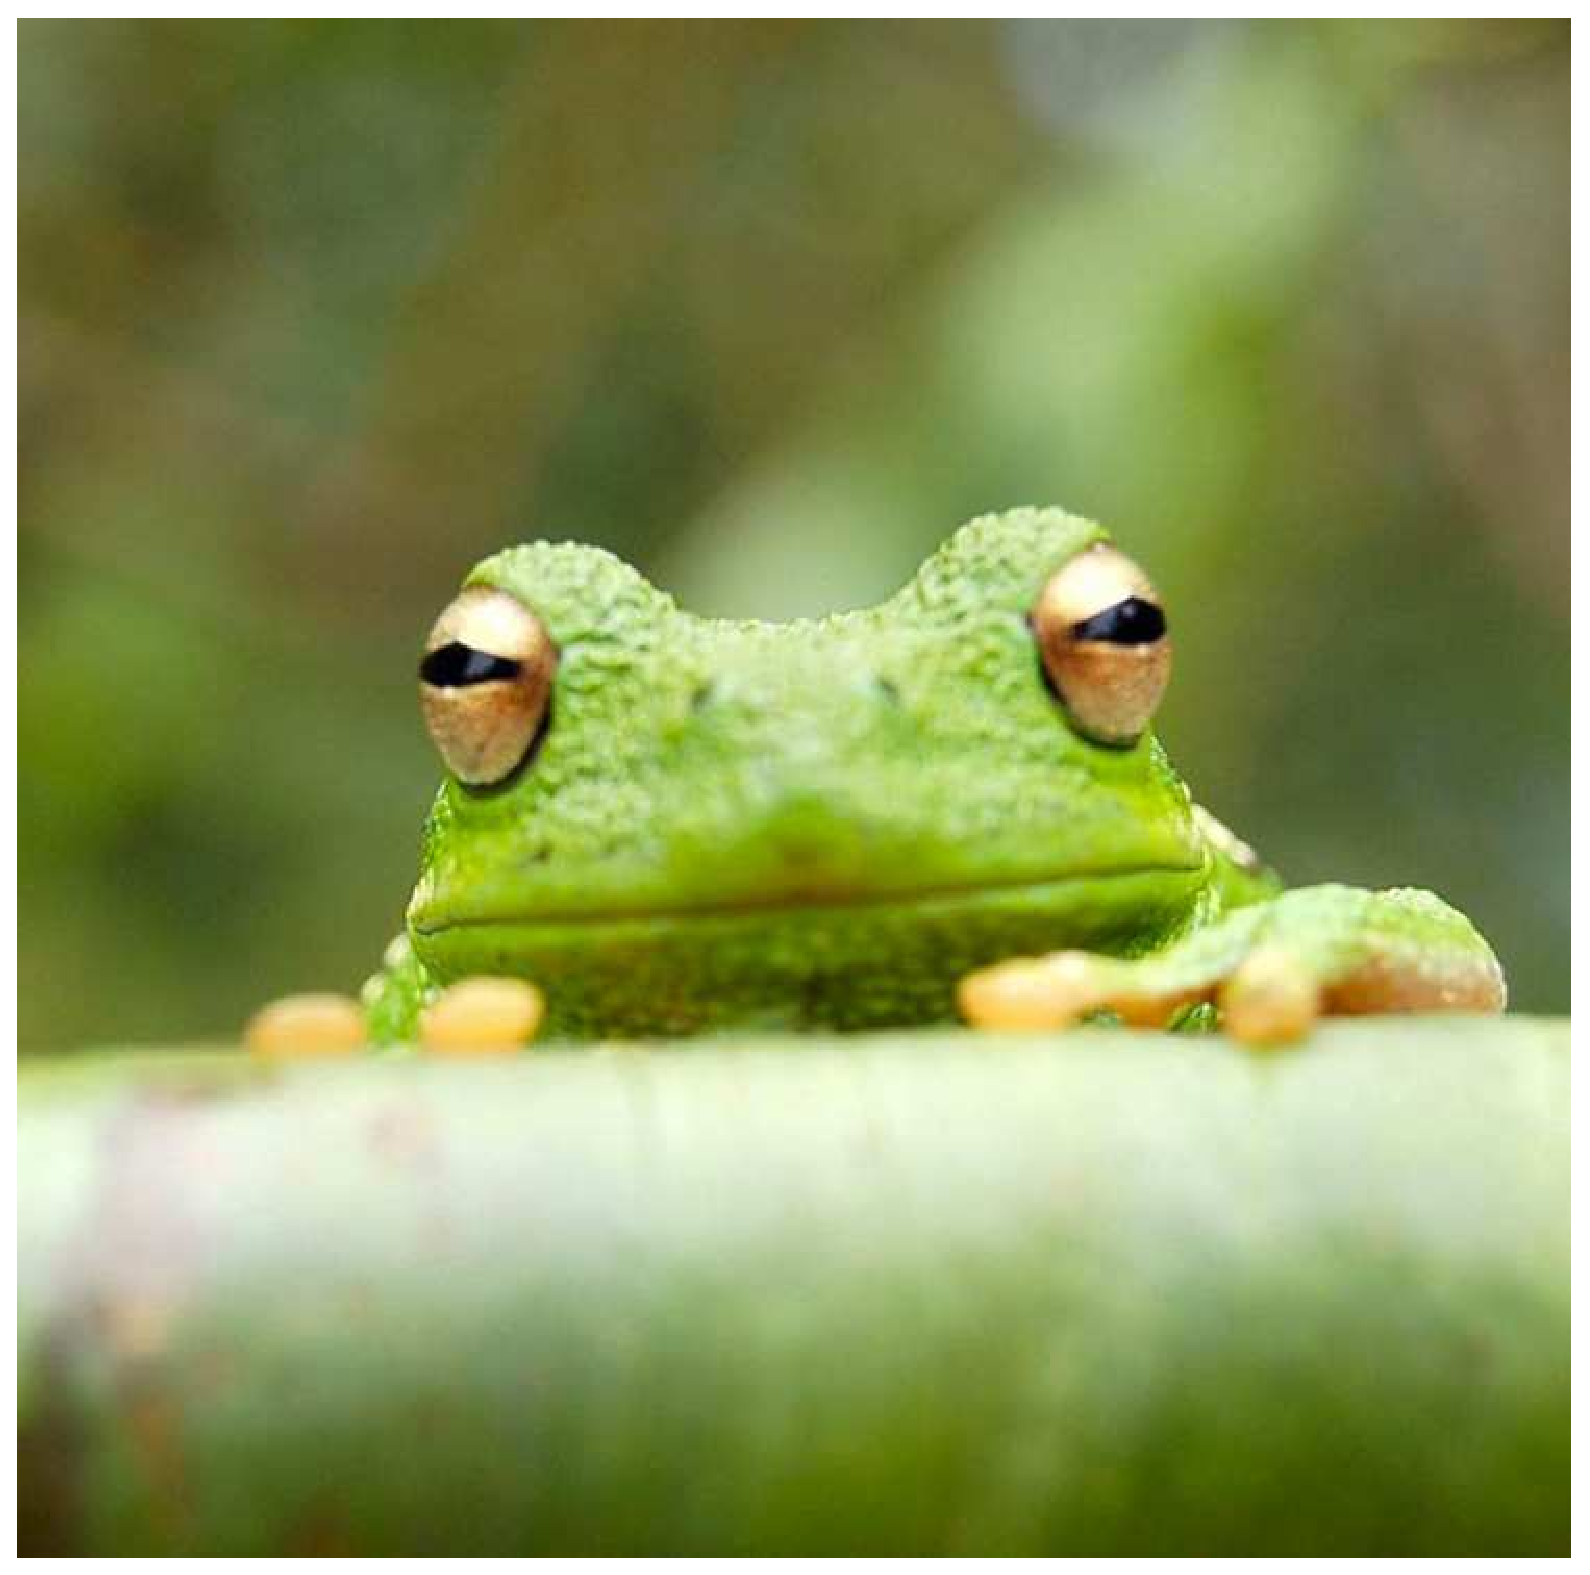
\includegraphics[width=.8\linewidth]{frog}
%\caption{Placeholder image of a frog with a long example caption to show justification setting.}
%\label{fig:frog}
%\end{figure}
%
%\subsection*{Digital Figures}
%\label{sec:figures}
%
%Figure \ref{fig:frog} shows an example of how to insert a column-wide figure. To insert a figure wider than one column, please use the \verb|\begin{figure*}...\end{figure*}| environment. Figures wider than one column should be sized to 11.4 cm or 17.8 cm wide.
%
%%% Do not use widetext if paper is in single column.
%\begin{widetext}
%\begin{align*}
%(x+y)^3&=(x+y)(x+y)^2\\
%       &=(x+y)(x^2+2xy+y^2) \numberthis \label{eqn:example} \\
%       &=x^3+3x^2y+3xy^3+x^3. 
%\end{align*}
%\end{widetext}

%\subsection*{Supporting Information (SI)}
%
%The main text of the paper must stand on its own without the SI. Refer to SI in the manuscript at an appropriate point in the text. Number supporting figures and tables starting with S1, S2, etc. Authors are limited to no more than 10 SI files, not including movie files. Authors who place detailed materials and methods in SI must provide sufficient detail in the main text methods to enable a reader to follow the logic of the procedures and results and also must reference the online methods. If a paper is fundamentally a study of a new method or technique, then the methods must be described completely in the main text. Because PNAS edits SI and composes it into a single PDF, authors must provide the following file formats only.


%\subsubsection*{SI Figures}


\matmethods{We here describe in detail our calculation of bin-averaged flux divergence profiles from GCM output.

For a GCM column at a given longitude, latitude, and time (we use monthly mean output), we must first identify a range of tropospheric model levels $k$ over which the temperature $T$ varies monotonically. We identify the uppermost of these levels \kmax\ as the minimum  $k>10$ for which $T[k+1]>T[k]$. If none such exists (i.e. no stratospheric inversion) then $\kmax$ takes its highest possible value (i.e. model top).
The minimum $k$ value $\kmin$ equals 1 if there is no inversion below \kmax, and otherwise is the largest $k< \kmax$ such that $T[k]>T[k-1]$. We then interpolate the column's SW and LW radiative fluxes over this $T$ range onto a uniform $T$ grid running from 150 to 350 K in increments of 2 K, and assign these interpolated profiles, weighted by column area,  to the appropriate \Ts\ bin using $T[1]$ (where \Ts-binning is done with the same uniform grid as for vertical levels $T$). We repeat this for each GCM column over the last 30 years of each simulation, keeping track of the accumulated column area for each bin and $T$ level. This allows us to produce an area-weighted average flux profile in each bin, where in a given bin the total area represented at each $T$ level drops off at lower and higher $T$  (due to small variations in $T[\kmin]$ and $T[\kmax]$ within the bin). These average flux profiles (one per bin) may then be differentiated with respect to $T$, yielding the $-\ppt \Fnet$ profiles shown in Fig. \ref{fnet_ipsl} and \ref{fnet_all}. To reduce noise in these figures, the profiles are cut off once the total area at a given $T$ is less than half of the maximum value in the vertical (where this maximum value is taken throughout most of that bin's tropospheric $T$ range, as expected). 

The decomposition of these net flux divergence profiles into their LW and SW components is given in Fig. S5, which shows that  \Ts-invariance aloft holds for the LW and SW separately in the GCMs, just as for the CRM.}


\showmatmethods % Display the Materials and Methods section

\acknow{Thanks are due to Tim Merlis, Mark Cane, Jake Seeley,  David Paynter, Yi Ming, and Leo Donner for helpful comments during various stages of this work, as well as to two anonymous reviewers for their close reading and thoughtful comments. This research used computing resources of the National Energy Research Scientific Computing Center (NERSC), which is supported by the Office of Science of the US Department of Energy under Contract DE-AC02-05CH11231.}

\showacknow % Display the acknowledgments section

% \pnasbreak splits and balances the columns before the references.
% If you see unexpected formatting errors, try commenting out this line
% as it can run into problems with floats and footnotes on the final page.
\pnasbreak

% Bibliography
\bibliography{library}


\end{document}